%!TEX TS-program = xelatex

\documentclass[t]{beamer}

\usetheme{Hannover}
\usecolortheme{rose}

%%% Работа с русским языком
\usepackage[english,russian]{babel}   %% загружает пакет многоязыковой вёрстки
\usepackage{fontspec,xltxtra,xunicode}      %% подготавливает загрузку шрифтов Open Type, True Type и др.
%\defaultfontfeatures{Ligatures={TeX},Renderer=Basic}  %% свойства шрифтов по умолчанию
\setmainfont[Ligatures={TeX,Historic},
SmallCapsFont={Brill},
SmallCapsFeatures={Letters=SmallCaps}]{Brill} %% задаёт основной шрифт документа
\setsansfont{Brill}                    %% задаёт шрифт без засечек
\setmonofont[Ligatures=NoCommon]{DejaVu Sans}
\newfontfamily\SYM{Brill}
\usepackage{indentfirst}
%%% Дополнительная работа с математикой
\usepackage{amsmath,amsfonts,amssymb,amsthm,mathtools} % AMS
\usepackage{icomma} % "Умная" запятая: $0,2$ --- число, $0, 2$ --- перечисление

%%% Работа с картинками
\usepackage{wrapfig} % Обтекание рисунков текстом
\usepackage{rotating}
\usepackage{fixltx2e}
\usepackage{hhline}
\usepackage{lscape}

%%% Работа с таблицами
\usepackage{array,tabularx,tabulary,booktabs} % Дополнительная работа с таблицами
\usepackage{longtable}  % Длинные таблицы
\usepackage{multirow} % Слияние строк в таблице

\usepackage{multicol} % Несколько колонок

%%% Страница
%\usepackage{fancyhdr} % Колонтитулы
% 	\pagestyle{fancy}
 	%\renewcommand{\headrulewidth}{0pt}  % Толщина линейки, отчеркивающей верхний колонтитул
% 	\lfoot{Нижний левый}
% 	\rfoot{Нижний правый}
% 	\rhead{Верхний правый}
% 	\chead{Верхний в центре}
% 	\lhead{Верхний левый}
%	\cfoot{Нижний в центре} % По умолчанию здесь номер страницы

\usepackage{setspace} % Интерлиньяж
%\onehalfspacing % Интерлиньяж 1.5
%\doublespacing % Интерлиньяж 2
\singlespacing % Интерлиньяж 1

\usepackage{subfig} % подкартинки
\usepackage{lastpage} % Узнать, сколько всего страниц в документе.
\usepackage{soul} % Модификаторы начертания
\usepackage{bbding}
\usepackage{hyperref}
\usepackage{tikz} % Работа с графикой
\usepackage{pgfplots}
\usepackage{pgfplotstable}
\usepackage{verbatim}

\usepackage{attachfile2}
 \attachfilesetup{appearance=true,
color=0 0 0
 }
\usepackage{alltt}

%%% Лингвистические пакеты
%\usepackage{savetrees} % пакет, который экономит место
\usepackage{forest} % для рисования деревьев
\usepackage{vowel} % для рисования трапеций гласных
\usepackage{natbib}
\bibpunct[: ]{[}{]}{;}{a}{}{,}
\usepackage[nogroupskip,nopostdot, nonumberlist]{glossaries}
%\usepackage{glossary-mcols} 
%\setglossarystyle{mcolindex}
\usepackage{philex} % пакет для примеров
\newcommand{\mytem}{\item[$\circ$]}
\addto\captionsrussian{
\renewcommand{\refname}{}}

\newcommand{\apostrophe}{\XeTeXglyph\XeTeXcharglyph"0027\relax}
\usetikzlibrary{patterns}

\usepackage{ulem}
\setbeamersize{text margin left=4mm,text margin right=1mm} 
\setbeamertemplate{navigation symbols}{
	\usebeamerfont{footline}%
    \usebeamercolor[fg]{footline}%
    \hspace{1em}%
    {{\small презентация доступна: \href{http://1drv.ms/1PMoiZj}{\textbf{http://1drv.ms/1PMoiZj}}}
    \hspace{40mm}
    \insertframenumber/\inserttotalframenumber\vspace{0.5mm}}}
% начало
\title[]{DiagrammeR}
\author[]{Г. Мороз}
\date{}
\begin{document}
\frame{\titlepage}
\section{узлы}
\begin{frame}[fragile]{DiagrammeR: создаем узлы}
\scriptsize
\begin{alltt}
library("DiagrammeR")
grViz("
digraph \{
      node [shape = box] \hfill # свойства узлов
      A \hfill # один узел
      \}
      ")
\end{alltt}
\normalsize
\end{frame}
\begin{frame}[fragile]{DiagrammeR: создаем узлы}

\includegraphics[width=\linewidth]{1.jpeg}
\end{frame}
\begin{frame}[fragile]{DiagrammeR: создаем узлы}
\scriptsize
\begin{alltt}
library("DiagrammeR")
grViz("
digraph \{
      node [shape = box] \hfill # свойства узлов
      A  \hfill # один узел
      {\color{red!13!blue}{B \hfill # второй узел
      C \hfill # третий узел}}
      \}
      ")
\end{alltt}
\normalsize
\end{frame}
\begin{frame}[fragile]{DiagrammeR: создаем узлы}
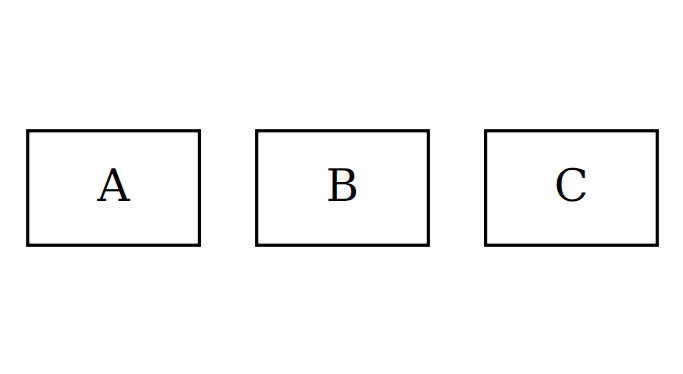
\includegraphics[width=\linewidth]{2.jpeg}
\end{frame}
\begin{frame}[fragile]{DiagrammeR: создаем узлы}
\scriptsize
\begin{alltt}
library("DiagrammeR")
grViz("
digraph \{
      node [shape = box] \hfill # свойства узлов
      A{\color{red!13!blue}{; B; С \hfill # можно через точку с запятой}}
      \}
      ")
\end{alltt}
\normalsize
\end{frame}
\begin{frame}[fragile]{DiagrammeR: создаем узлы}
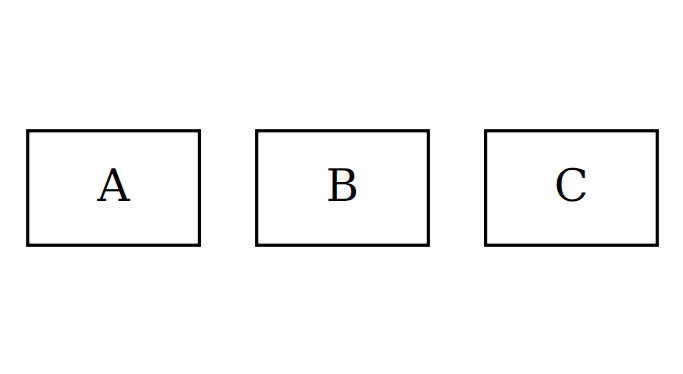
\includegraphics[width=\linewidth]{2.jpeg}
\end{frame}
\section{ребра}
\begin{frame}[fragile]{DiagrammeR: создаем ребра}
\scriptsize
\begin{alltt}
library("DiagrammeR")
grViz("
digraph \{
      node [shape = box] \hfill # свойства узлов
      A; B; C \hfill # можно через точку с запятой
      {\color{red!13!blue}{A -> B \hfill создаем ребро}}
      \}
      ")
\end{alltt}
\normalsize
\end{frame}
\begin{frame}[fragile]{DiagrammeR: создаем ребра}
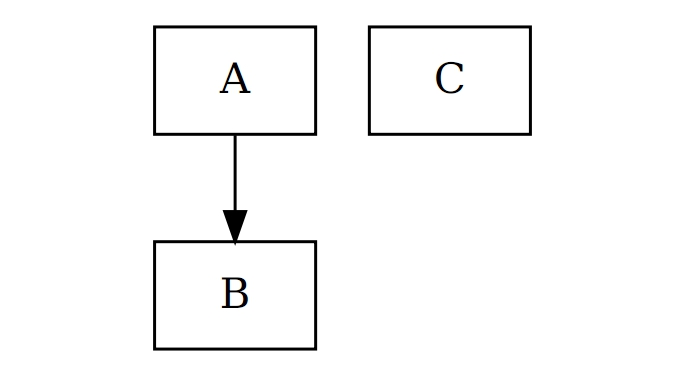
\includegraphics[width=\linewidth]{3.jpeg}
\end{frame}

\begin{frame}[fragile]{DiagrammeR: создаем ребра}
\scriptsize
\begin{alltt}
library("DiagrammeR")
grViz("
digraph \{
      node [shape = box] \hfill # свойства узлов
      A; B; C \hfill # можно через точку с запятой
      A -> B {\color{red!13!blue}{B -> A \hfill создаем ребро}}
      \}
      ")
\end{alltt}
\normalsize
\end{frame}
\begin{frame}[fragile]{DiagrammeR: создаем ребра}
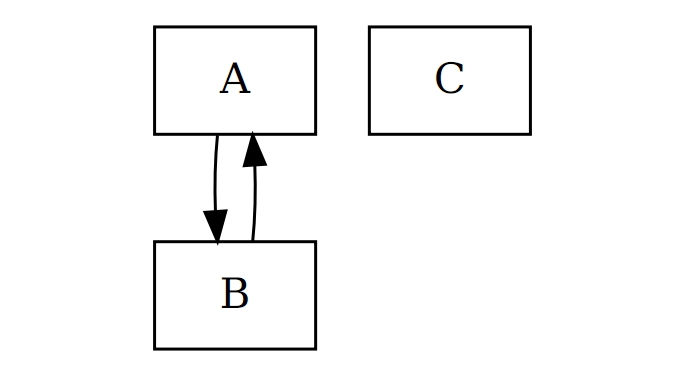
\includegraphics[width=\linewidth]{4.jpeg}
\end{frame}

\begin{frame}[fragile]{DiagrammeR: создаем ребра}
\scriptsize
\begin{alltt}
library("DiagrammeR")
grViz("
digraph \{
      node [shape = box] \hfill # свойства узлов
      A; B; C \hfill # можно через точку с запятой
      A -> B B -> A {\color{red!13!blue}{ A -> C\hfill создаем ребро}}
      \}
      ")
\end{alltt}
\normalsize
\end{frame}
\begin{frame}[fragile]{DiagrammeR: создаем ребра}
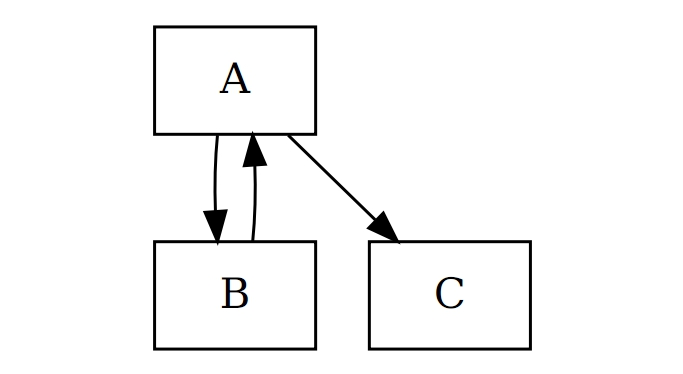
\includegraphics[width=\linewidth]{5.jpeg}
\end{frame}

\begin{frame}[fragile]{DiagrammeR: создаем ребра}
\scriptsize
\begin{alltt}
library("DiagrammeR")
grViz("
digraph \{
      node [shape = box] \hfill # свойства узлов
      A; B; C \hfill # можно через точку с запятой
      {\color{red!13!blue}{A -> \{B, C\} }} B -> A \hfill{\color{red!13!blue}{ создаем ребро}}
      \}
      ")
\end{alltt}
\normalsize
\end{frame}
\begin{frame}[fragile]{DiagrammeR: создаем ребра}
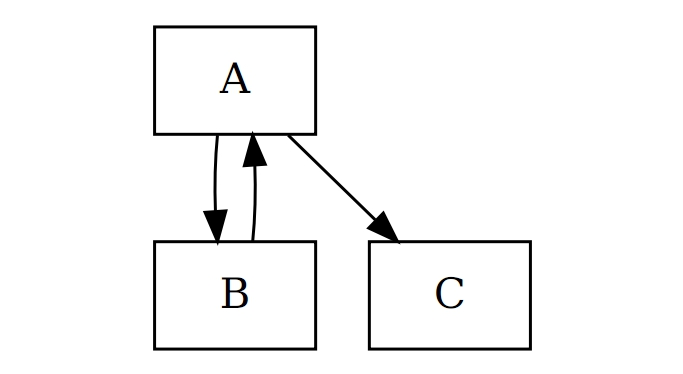
\includegraphics[width=\linewidth]{5.jpeg}
\end{frame}

\begin{frame}[fragile]{DiagrammeR: создаем ребра}
\scriptsize
\begin{alltt}
library("DiagrammeR")
grViz("
digraph \{
      node [shape = box] \hfill # свойства узлов
      A; B; C \hfill # можно через точку с запятой
      A -> \{B, C\} B -> A {\color{red!13!blue}{C -> C \hfill создаем ребро}}
      \}
      ")
\end{alltt}
\normalsize
\end{frame}
\begin{frame}[fragile]{DiagrammeR: создаем ребра}
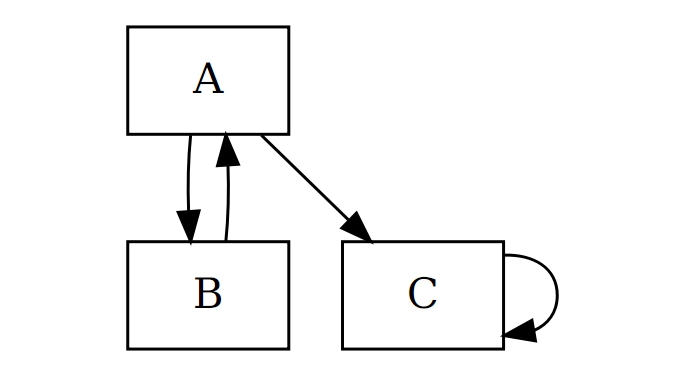
\includegraphics[width=\linewidth]{6.jpeg}
\end{frame}

\begin{frame}[fragile]{DiagrammeR: создаем ребра}
\scriptsize
\begin{alltt}
library("DiagrammeR")
grViz("
digraph \{
      node [shape = box] \hfill # свойства узлов
      A; B; C \hfill # можно через точку с запятой
      A -> \{B, C\} B -> A C -> C {\color{red!13!blue}{C -> B \hfill создаем ребро}}
      \}
      ")
\end{alltt}
\normalsize
\end{frame}
\begin{frame}[fragile]{DiagrammeR: создаем ребра}
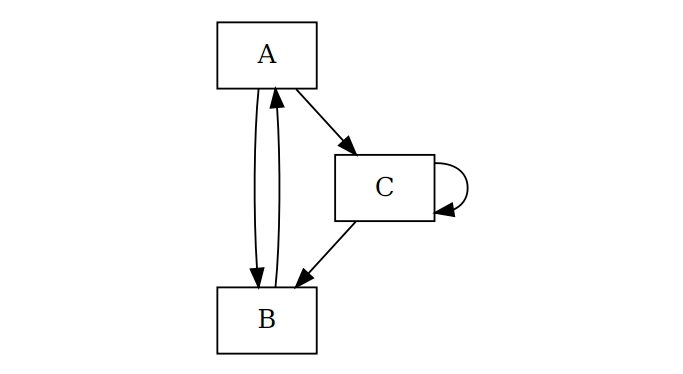
\includegraphics[width=\linewidth]{7.jpeg}
\end{frame}
\section{атриб. узла}
\begin{frame}[fragile]{DiagrammeR: shape = box}
\scriptsize
\begin{alltt}
library("DiagrammeR")
grViz("
digraph \{
      node [{\color{red!13!blue}{shape = box}}] \hfill # форма узлов
      A; B; C \hfill # можно через точку с запятой
      A -> \{B, C\} B -> A C -> C C -> B \hfill создаем ребро
      \}
      ")
\end{alltt}
\normalsize
\end{frame}
\begin{frame}[fragile]{DiagrammeR: shape = box}
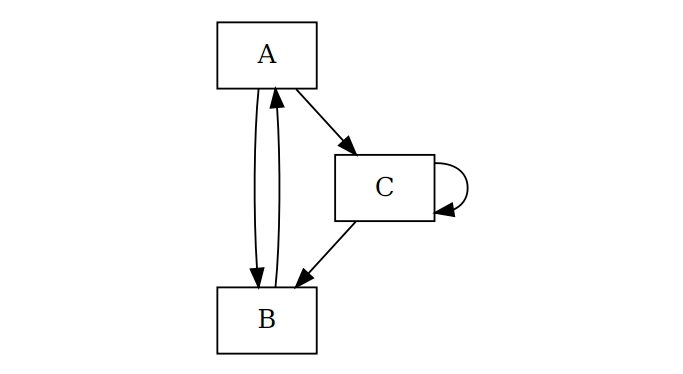
\includegraphics[width=\linewidth]{7.jpeg}
\end{frame}

\begin{frame}[fragile]{DiagrammeR: shape = square}
\scriptsize
\begin{alltt}
library("DiagrammeR")
grViz("
digraph \{
      node [{\color{red!13!blue}{shape = square}}] \hfill # форма узлов
      A; B; C \hfill # можно через точку с запятой
      A -> \{B, C\} B -> A C -> C C -> B \hfill создаем ребро
      \}
      ")
\end{alltt}
\normalsize
\end{frame}
\begin{frame}[fragile]{DiagrammeR: shape = square}
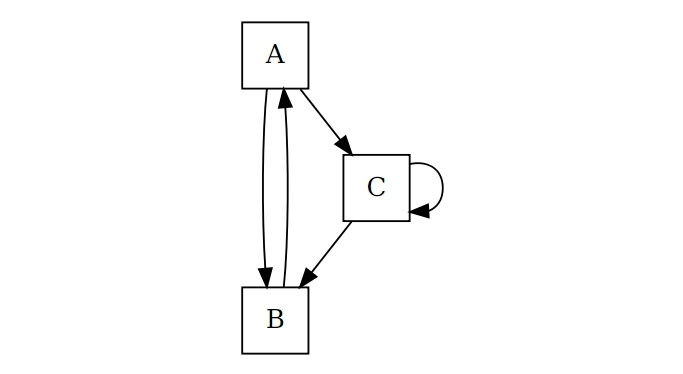
\includegraphics[width=\linewidth]{10.jpeg}
\end{frame}

\begin{frame}[fragile]{DiagrammeR: shape = circle}
\scriptsize
\begin{alltt}
library("DiagrammeR")
grViz("
digraph \{
      node [{\color{red!13!blue}{shape = circle}}] \hfill # форма узлов
      A; B; C \hfill # можно через точку с запятой
      A -> \{B, C\} B -> A C -> C C -> B \hfill создаем ребро
      \}
      ")
\end{alltt}
\normalsize
\end{frame}
\begin{frame}[fragile]{DiagrammeR: shape = circle}
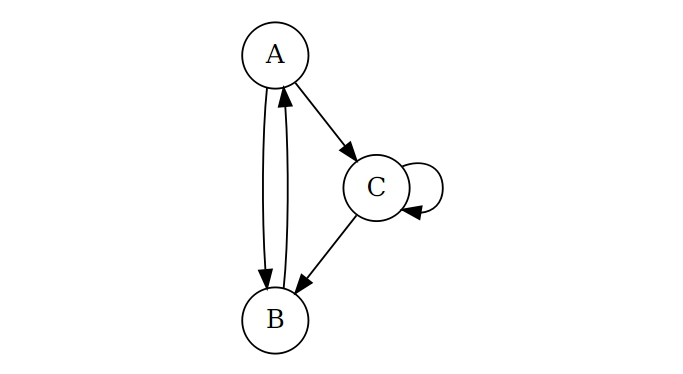
\includegraphics[width=\linewidth]{8.jpeg}
\end{frame}

\begin{frame}[fragile]{DiagrammeR: shape = ellipse}
\scriptsize
\begin{alltt}
library("DiagrammeR")
grViz("
digraph \{
      node [{\color{red!13!blue}{shape = ellipse}}] \hfill # форма узлов
      A; B; C \hfill # можно через точку с запятой
      A -> \{B, C\} B -> A C -> C C -> B \hfill создаем ребро
      \}
      ")
\end{alltt}
\normalsize
\end{frame}
\begin{frame}[fragile]{DiagrammeR: shape = ellipse}
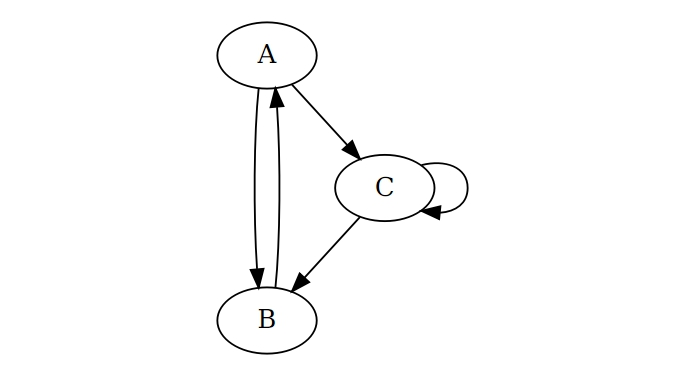
\includegraphics[width=\linewidth]{12.jpeg}
\end{frame}

\begin{frame}[fragile]{DiagrammeR: shape = egg}
\scriptsize
\begin{alltt}
library("DiagrammeR")
grViz("
digraph \{
      node [{\color{red!13!blue}{shape = egg}}] \hfill # форма узлов
      A; B; C \hfill # можно через точку с запятой
      A -> \{B, C\} B -> A C -> C C -> B \hfill создаем ребро
      \}
      ")
\end{alltt}
\normalsize
\end{frame}
\begin{frame}[fragile]{DiagrammeR: shape = egg}
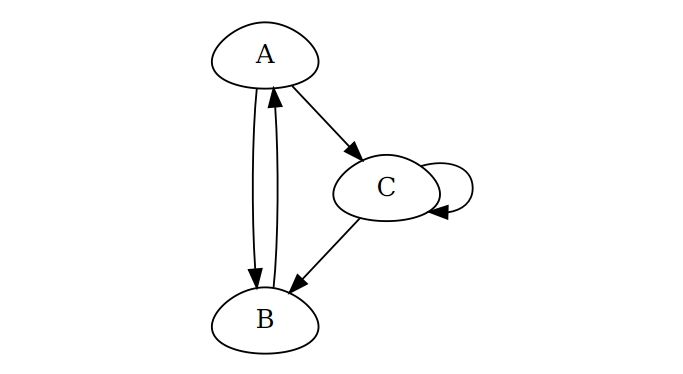
\includegraphics[width=\linewidth]{14.jpeg}
\end{frame}

\begin{frame}[fragile]{DiagrammeR: shape = diamond}
\scriptsize
\begin{alltt}
library("DiagrammeR")
grViz("
digraph \{
      node [{\color{red!13!blue}{shape = diamond}}] \hfill # форма узлов
      A; B; C \hfill # можно через точку с запятой
      A -> \{B, C\} B -> A C -> C C -> B \hfill создаем ребро
      \}
      ")
\end{alltt}
\normalsize
\end{frame}
\begin{frame}[fragile]{DiagrammeR: shape = diamond}
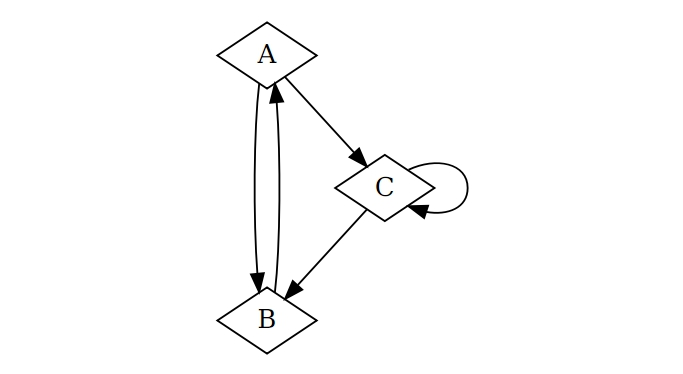
\includegraphics[width=\linewidth]{11.jpeg}
\end{frame}

\begin{frame}[fragile]{DiagrammeR: shape = triangle}
\scriptsize
\begin{alltt}
library("DiagrammeR")
grViz("
digraph \{
      node [{\color{red!13!blue}{shape = triangle}}] \hfill # форма узлов
      A; B; C \hfill # можно через точку с запятой
      A -> \{B, C\} B -> A C -> C C -> B \hfill создаем ребро
      \}
      ")
\end{alltt}
\normalsize
\end{frame}
\begin{frame}[fragile]{DiagrammeR: shape = triangle}
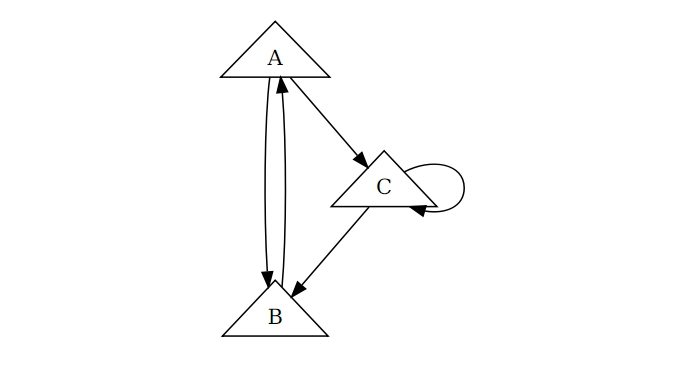
\includegraphics[width=\linewidth]{13.jpeg}
\end{frame}

\begin{frame}[fragile]{DiagrammeR: shape = point}
\scriptsize
\begin{alltt}
library("DiagrammeR")
grViz("
digraph \{
      node [{\color{red!13!blue}{shape = point}}] \hfill # форма узлов
      A; B; C \hfill # можно через точку с запятой
      A -> \{B, C\} B -> A C -> C C -> B \hfill создаем ребро
      \}
      ")
\end{alltt}
\normalsize
\end{frame}
\begin{frame}[fragile]{DiagrammeR: shape = point}
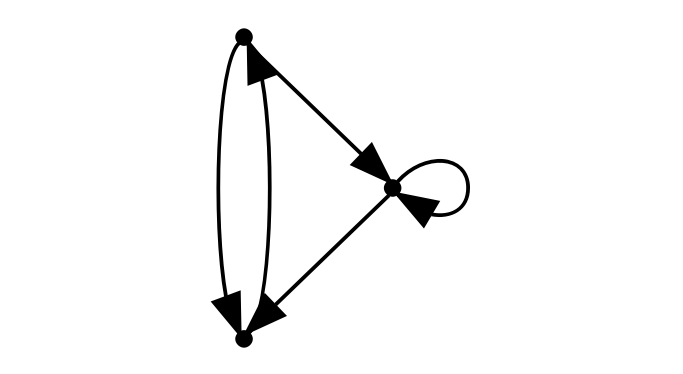
\includegraphics[width=\linewidth]{9.jpeg}
\end{frame}

\begin{frame}[fragile]{DiagrammeR: shape = plaintext}
\scriptsize
\begin{alltt}
library("DiagrammeR")
grViz("
digraph \{
      node [{\color{red!13!blue}{shape = plaintext}}] \hfill # форма узлов
      A; B; C \hfill # можно через точку с запятой
      A -> \{B, C\} B -> A C -> C C -> B \hfill создаем ребро
      \}
      ")
\end{alltt}
\normalsize
\end{frame}
\begin{frame}[fragile]{DiagrammeR: shape = plaintext}
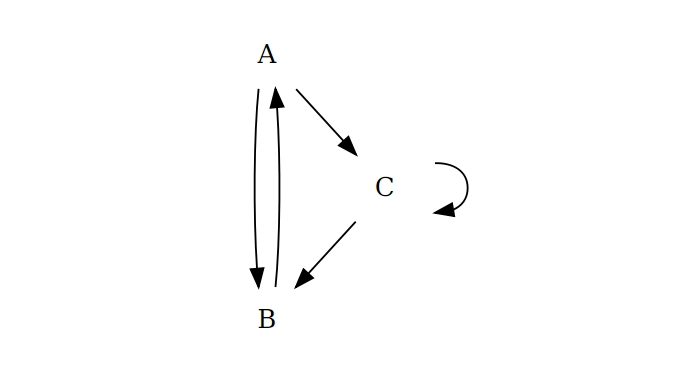
\includegraphics[width=\linewidth]{15.jpeg}
\end{frame}

\begin{frame}[fragile]{DiagrammeR: color = red}
\scriptsize
\begin{alltt}
library("DiagrammeR")
grViz("
digraph \{
      node [shape = egg, \hfill # форма узлов
      {\color{red!13!blue}{color = red}}] \hfill # цвет узлов
      A; B; C \hfill # можно через точку с запятой
      A -> \{B, C\} B -> A C -> C C -> B \hfill создаем ребро
      \}
      ")
\end{alltt}
\normalsize
\end{frame}
\begin{frame}[fragile]{DiagrammeR: color = red}
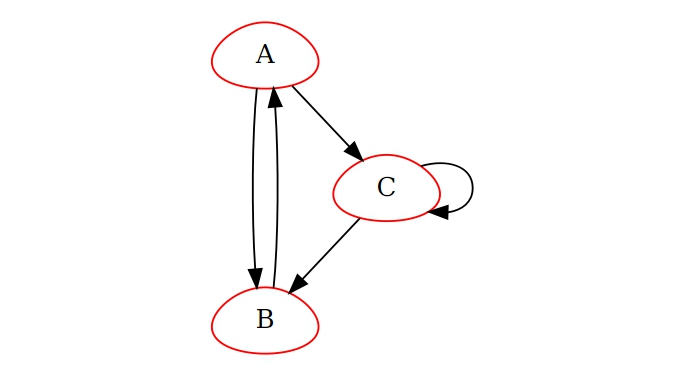
\includegraphics[width=\linewidth]{16.jpeg}
\end{frame}

\begin{frame}[fragile]{DiagrammeR: fontcolor = red}
\scriptsize
\begin{alltt}
library("DiagrammeR")
grViz("
digraph \{
      node [shape = egg, \hfill # форма узлов
      {\color{red!13!blue}{fontcolor = red}}] \hfill # цвет имени узла
      A; B; C \hfill # можно через точку с запятой
      A -> \{B, C\} B -> A C -> C C -> B \hfill создаем ребро
      \}
      ")
\end{alltt}
\normalsize
\end{frame}
\begin{frame}[fragile]{DiagrammeR: fontcolor = red}
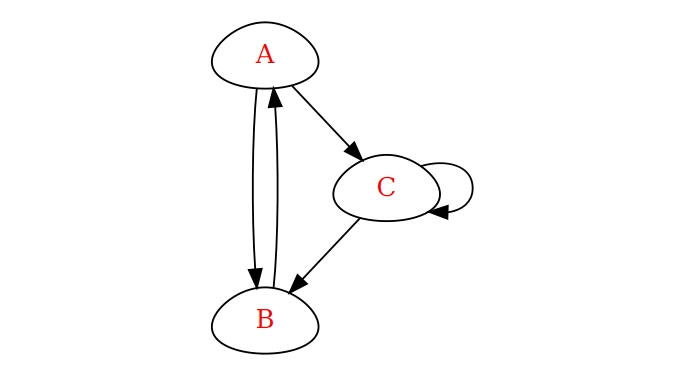
\includegraphics[width=\linewidth]{17.jpeg}
\end{frame}

\begin{frame}[fragile]{DiagrammeR: style = dotted}
\scriptsize
\begin{alltt}
library("DiagrammeR")
grViz("
digraph \{
      node [shape = egg, \hfill # форма узлов
			      fontcolor = red, \hfill # цвет имени узла
      {\color{red!13!blue}{style = dotted}}] \hfill # тип границы
      A; B; C \hfill # можно через точку с запятой
      A -> \{B, C\} B -> A C -> C C -> B \hfill создаем ребро
      \}
      ")
\end{alltt}
\normalsize
\end{frame}
\begin{frame}[fragile]{DiagrammeR: style = dotted}
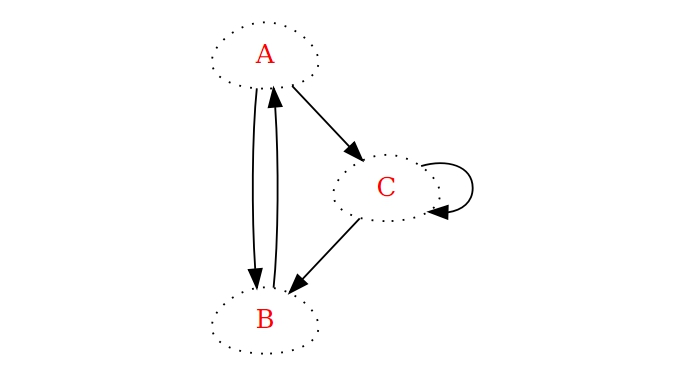
\includegraphics[width=\linewidth]{18.jpeg}
\end{frame}

\begin{frame}[fragile]{DiagrammeR: style = dashed}
\scriptsize
\begin{alltt}
library("DiagrammeR")
grViz("
digraph \{
      node [shape = egg, \hfill # форма узлов
			      fontcolor = red, \hfill # цвет имени узла
      {\color{red!13!blue}{style = dashed}}] \hfill # тип границы
      A; B; C \hfill # можно через точку с запятой
      A -> \{B, C\} B -> A C -> C C -> B \hfill создаем ребро
      \}
      ")
\end{alltt}
\normalsize
\end{frame}
\begin{frame}[fragile]{DiagrammeR: style = dashed}
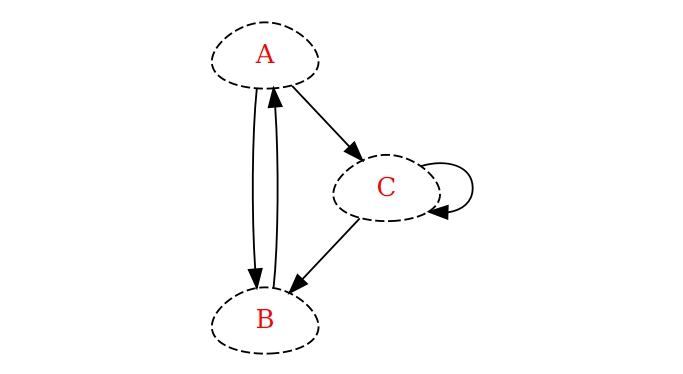
\includegraphics[width=\linewidth]{19.jpeg}
\end{frame}

\begin{frame}[fragile]{DiagrammeR: style = filled}
\scriptsize
\begin{alltt}
library("DiagrammeR")
grViz("
digraph \{
      node [shape = egg, \hfill # форма узлов
			      fontcolor = red, \hfill # цвет имени узла
      {\color{red!13!blue}{style = filled}}] \hfill # тип
      A; B; C \hfill # можно через точку с запятой
      A -> \{B, C\} B -> A C -> C C -> B \hfill создаем ребро
      \}
      ")
\end{alltt}
\normalsize
\end{frame}
\begin{frame}[fragile]{DiagrammeR: style = filled}
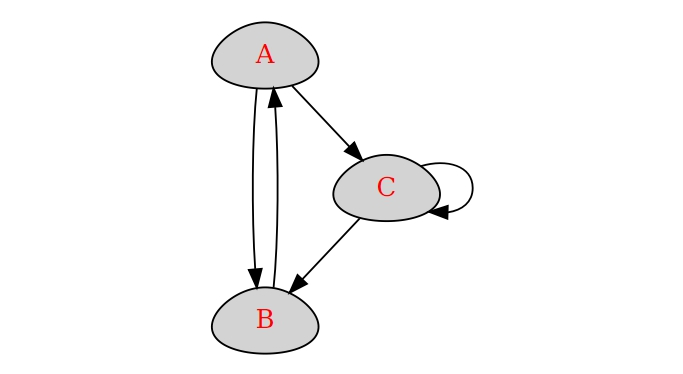
\includegraphics[width=\linewidth]{20.jpeg}
\end{frame}

\begin{frame}[fragile]{DiagrammeR: fillcolor = lightblue}
\scriptsize
\begin{alltt}
library("DiagrammeR")
grViz("
digraph \{
      node [shape = egg, \hfill # форма узлов
			      fontcolor = red, \hfill # цвет имени узла
			      style = filled, # тип
      {\color{red!13!blue}{fillcolor = lightblue}}] \hfill # цвет заполнения
      A; B; C \hfill # можно через точку с запятой
      A -> \{B, C\} B -> A C -> C C -> B \hfill создаем ребро
      \}
      ")
\end{alltt}
\normalsize
\end{frame}
\begin{frame}[fragile]{DiagrammeR: fillcolor = lightblue}
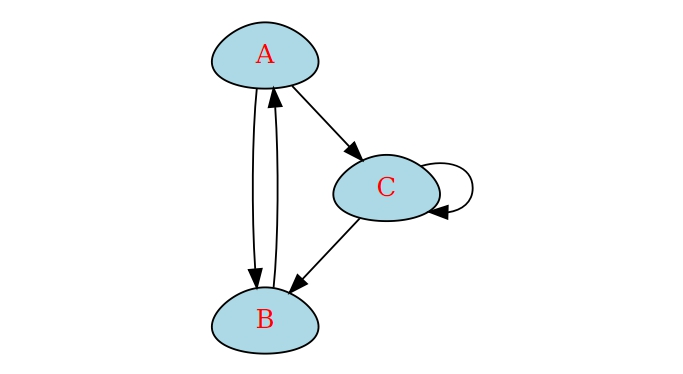
\includegraphics[width=\linewidth]{21.jpeg}
\end{frame}

\section{атриб. линии}
\begin{frame}[fragile]{DiagrammeR: color = green}
\scriptsize
\begin{alltt}
library("DiagrammeR")
grViz("
digraph \{
      node [shape = egg, \hfill # форма узлов
			      fontcolor = red, \hfill # цвет имени узла
			      style = filled, # тип
      fillcolor = lightblue] \hfill # цвет заполнения
      A; B; C \hfill # можно через точку с запятой
{\color{red!13!blue}{      edge [color = black] \hfill # цвет ребра}}
      A -> {B, C}
{\color{red!13!blue}{      edge [color = blue]   \hfill # цвет ребра}}
      B -> A 
{\color{red!13!blue}{      edge [color = green] \hfill # цвет ребра}}
      C -> C C -> B
      \}
      ")
\end{alltt}
\normalsize
\end{frame}
\begin{frame}[fragile]{DiagrammeR: color = green}
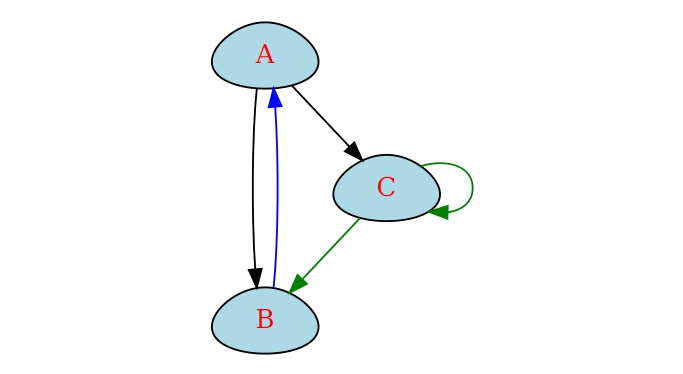
\includegraphics[width=\linewidth]{22.jpeg}
\end{frame}

\begin{frame}[fragile]{DiagrammeR: arrowhead = box}
\scriptsize
\begin{alltt}
library("DiagrammeR")
grViz("
digraph \{
      node [shape = egg, \hfill # форма узлов
			      fontcolor = red, \hfill # цвет имени узла
			      style = filled, # тип
      fillcolor = lightblue] \hfill # цвет заполнения
      A; B; C \hfill # можно через точку с запятой
      edge [color = black, \hfill # цвет ребра
{\color{red!13!blue}{                 arrowhead = box] \hfill # конец ребра}}
      A -> {B, C}
      edge [color = blue]   \hfill # цвет ребра
      B -> A 
      edge [color = green] \hfill # цвет ребра
      C -> C C -> B
      \}
      ")
\end{alltt}
\normalsize
\end{frame}
\begin{frame}[fragile]{DiagrammeR: arrowhead = box}
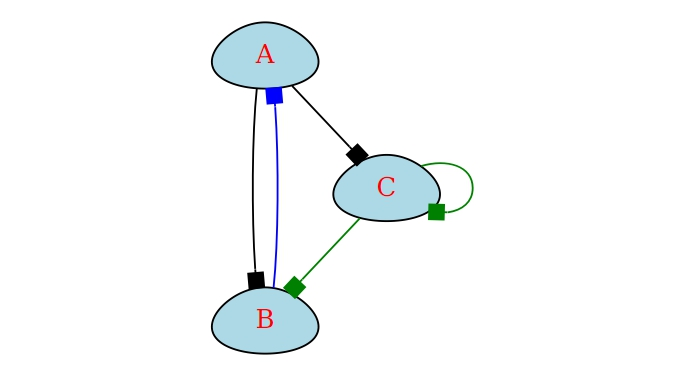
\includegraphics[width=\linewidth]{23.jpeg}
\end{frame}

\begin{frame}[fragile]{DiagrammeR: arrowhead = crow}
\scriptsize
\begin{alltt}
library("DiagrammeR")
grViz("
digraph \{
      node [shape = egg, \hfill # форма узлов
			      fontcolor = red, \hfill # цвет имени узла
			      style = filled, # тип
      fillcolor = lightblue] \hfill # цвет заполнения
      A; B; C \hfill # можно через точку с запятой
      edge [color = black, \hfill # цвет ребра
{\color{red!13!blue}{                 arrowhead = crow] \hfill # конец ребра}}
      A -> {B, C}
      edge [color = blue]   \hfill # цвет ребра
      B -> A 
      edge [color = green] \hfill # цвет ребра
      C -> C C -> B
      \}
      ")
\end{alltt}
\normalsize
\end{frame}
\begin{frame}[fragile]{DiagrammeR: arrowhead = crow}
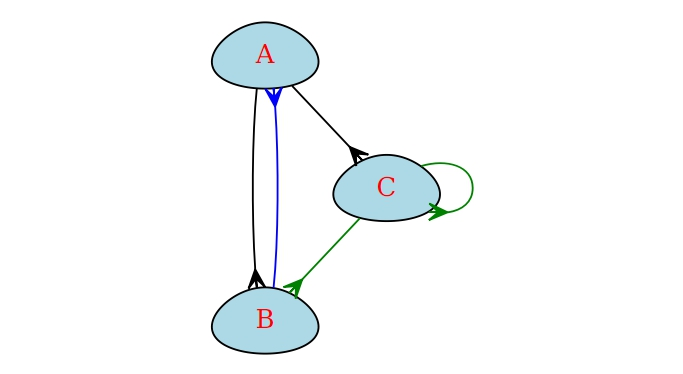
\includegraphics[width=\linewidth]{24.jpeg}
\end{frame}

\begin{frame}[fragile]{DiagrammeR: arrowhead = curve}
\scriptsize
\begin{alltt}
library("DiagrammeR")
grViz("
digraph \{
      node [shape = egg, \hfill # форма узлов
			      fontcolor = red, \hfill # цвет имени узла
			      style = filled, # тип
      fillcolor = lightblue] \hfill # цвет заполнения
      A; B; C \hfill # можно через точку с запятой
      edge [color = black, \hfill # цвет ребра
{\color{red!13!blue}{                 arrowhead = curve] \hfill # конец ребра}}
      A -> {B, C}
      edge [color = blue]   \hfill # цвет ребра
      B -> A 
      edge [color = green] \hfill # цвет ребра
      C -> C C -> B
      \}
      ")
\end{alltt}
\normalsize
\end{frame}
\begin{frame}[fragile]{DiagrammeR: arrowhead = curve}
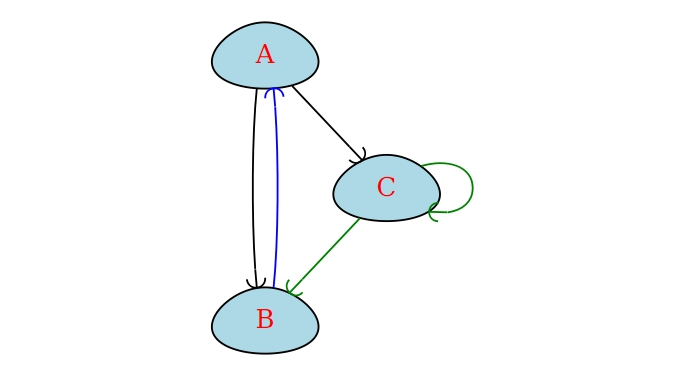
\includegraphics[width=\linewidth]{25.jpeg}
\end{frame}

\begin{frame}[fragile]{DiagrammeR: arrowhead = diamond}
\scriptsize
\begin{alltt}
library("DiagrammeR")
grViz("
digraph \{
      node [shape = egg, \hfill # форма узлов
			      fontcolor = red, \hfill # цвет имени узла
			      style = filled, # тип
      fillcolor = lightblue] \hfill # цвет заполнения
      A; B; C \hfill # можно через точку с запятой
      edge [color = black, \hfill # цвет ребра
{\color{red!13!blue}{                 arrowhead = diamond] \hfill # конец ребра}}
      A -> {B, C}
      edge [color = blue]   \hfill # цвет ребра
      B -> A 
      edge [color = green] \hfill # цвет ребра
      C -> C C -> B
      \}
      ")
\end{alltt}
\normalsize
\end{frame}
\begin{frame}[fragile]{DiagrammeR: arrowhead = diamond}
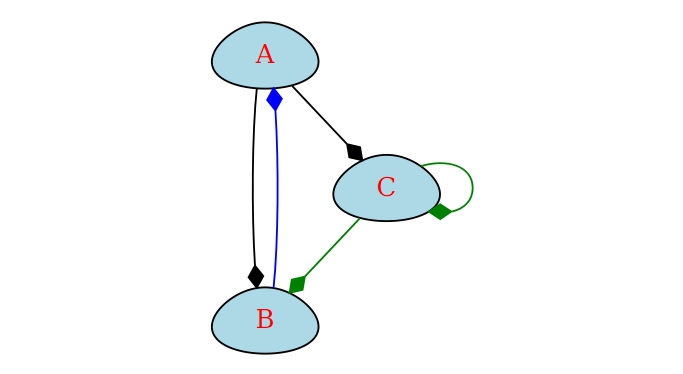
\includegraphics[width=\linewidth]{26.jpeg}
\end{frame}

\begin{frame}[fragile]{DiagrammeR: arrowhead = dot}
\scriptsize
\begin{alltt}
library("DiagrammeR")
grViz("
digraph \{
      node [shape = egg, \hfill # форма узлов
			      fontcolor = red, \hfill # цвет имени узла
			      style = filled, # тип
      fillcolor = lightblue] \hfill # цвет заполнения
      A; B; C \hfill # можно через точку с запятой
      edge [color = black, \hfill # цвет ребра
{\color{red!13!blue}{                 arrowhead = dot] \hfill # конец ребра}}
      A -> {B, C}
      edge [color = blue]   \hfill # цвет ребра
      B -> A 
      edge [color = green] \hfill # цвет ребра
      C -> C C -> B
      \}
      ")
\end{alltt}
\normalsize
\end{frame}
\begin{frame}[fragile]{DiagrammeR: arrowhead = dot}
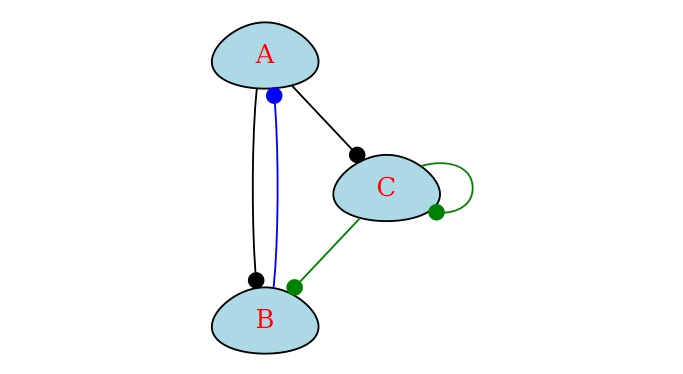
\includegraphics[width=\linewidth]{27.jpeg}
\end{frame}

\begin{frame}[fragile]{DiagrammeR: arrowhead = inv}
\scriptsize
\begin{alltt}
library("DiagrammeR")
grViz("
digraph \{
      node [shape = egg, \hfill # форма узлов
			      fontcolor = red, \hfill # цвет имени узла
			      style = filled, # тип
      fillcolor = lightblue] \hfill # цвет заполнения
      A; B; C \hfill # можно через точку с запятой
      edge [color = black, \hfill # цвет ребра
{\color{red!13!blue}{                 arrowhead = inv] \hfill # конец ребра}}
      A -> {B, C}
      edge [color = blue]   \hfill # цвет ребра
      B -> A 
      edge [color = green] \hfill # цвет ребра
      C -> C C -> B
      \}
      ")
\end{alltt}
\normalsize
\end{frame}
\begin{frame}[fragile]{DiagrammeR: arrowhead = inv}
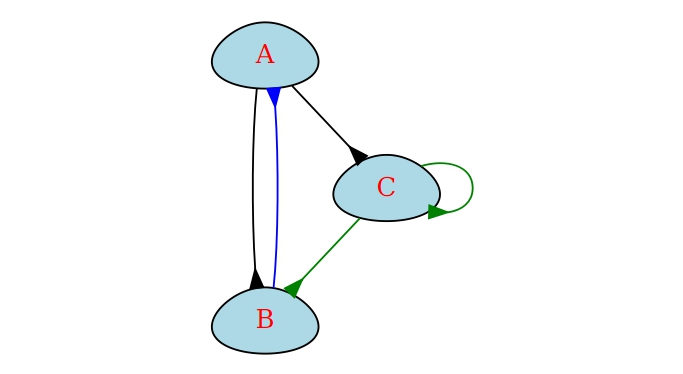
\includegraphics[width=\linewidth]{28.jpeg}
\end{frame}

\begin{frame}[fragile]{DiagrammeR: arrowhead = none}
\scriptsize
\begin{alltt}
library("DiagrammeR")
grViz("
digraph \{
      node [shape = egg, \hfill # форма узлов
			      fontcolor = red, \hfill # цвет имени узла
			      style = filled, # тип
      fillcolor = lightblue] \hfill # цвет заполнения
      A; B; C \hfill # можно через точку с запятой
      edge [color = black, \hfill # цвет ребра
{\color{red!13!blue}{                 arrowhead = none] \hfill # конец ребра}}
      A -> {B, C}
      edge [color = blue]   \hfill # цвет ребра
      B -> A 
      edge [color = green] \hfill # цвет ребра
      C -> C C -> B
      \}
      ")
\end{alltt}
\normalsize
\end{frame}
\begin{frame}[fragile]{DiagrammeR: arrowhead = none}
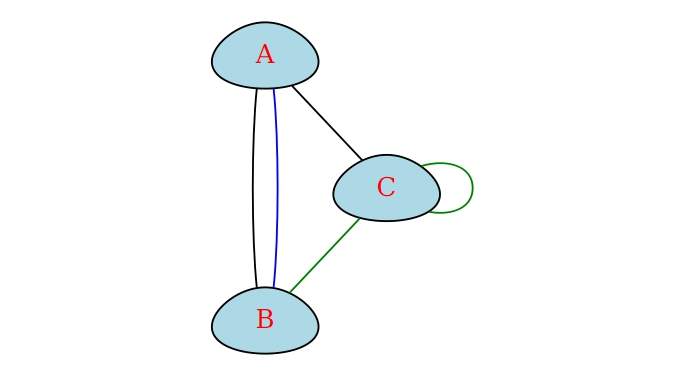
\includegraphics[width=\linewidth]{29.jpeg}
\end{frame}

\begin{frame}[fragile]{DiagrammeR: arrowhead = tee}
\scriptsize
\begin{alltt}
library("DiagrammeR")
grViz("
digraph \{
      node [shape = egg, \hfill # форма узлов
			      fontcolor = red, \hfill # цвет имени узла
			      style = filled, # тип
      fillcolor = lightblue] \hfill # цвет заполнения
      A; B; C \hfill # можно через точку с запятой
      edge [color = black, \hfill # цвет ребра
{\color{red!13!blue}{                 arrowhead = tee] \hfill # конец ребра}}
      A -> {B, C}
      edge [color = blue]   \hfill # цвет ребра
      B -> A 
      edge [color = green] \hfill # цвет ребра
      C -> C C -> B
      \}
      ")
\end{alltt}
\normalsize
\end{frame}
\begin{frame}[fragile]{DiagrammeR: arrowhead = tee}
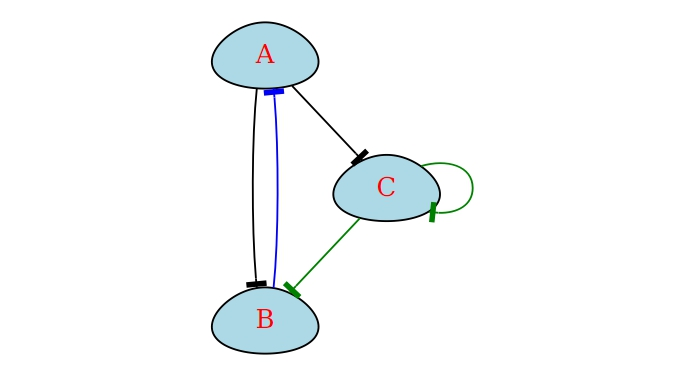
\includegraphics[width=\linewidth]{30.jpeg}
\end{frame}

\begin{frame}[fragile]{DiagrammeR: arrowhead = vee}
\scriptsize
\begin{alltt}
library("DiagrammeR")
grViz("
digraph \{
      node [shape = egg, \hfill # форма узлов
			      fontcolor = red, \hfill # цвет имени узла
			      style = filled, # тип
      fillcolor = lightblue] \hfill # цвет заполнения
      A; B; C \hfill # можно через точку с запятой
      edge [color = black, \hfill # цвет ребра
{\color{red!13!blue}{                 arrowhead = vee] \hfill # конец ребра}}
      A -> {B, C}
      edge [color = blue]   \hfill # цвет ребра
      B -> A 
      edge [color = green] \hfill # цвет ребра
      C -> C C -> B
      \}
      ")
\end{alltt}
\normalsize
\end{frame}
\begin{frame}[fragile]{DiagrammeR: arrowhead = vee}
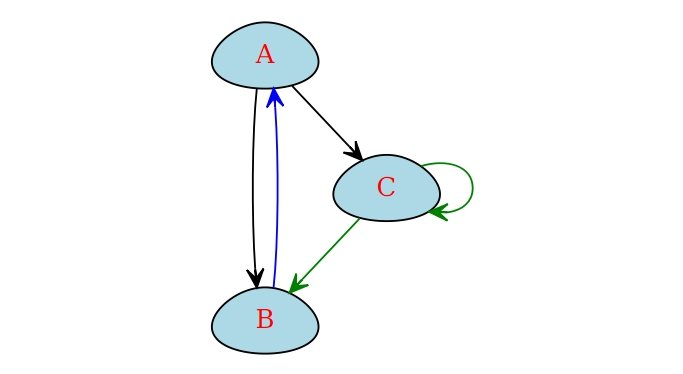
\includegraphics[width=\linewidth]{31.jpeg}
\end{frame}

\begin{frame}[fragile]{DiagrammeR: style = dotted}
\scriptsize
\begin{alltt}
library("DiagrammeR")
grViz("
digraph \{
      node [shape = egg, \hfill # форма узлов
			      fontcolor = red, \hfill # цвет имени узла
			      style = filled, # тип
      fillcolor = lightblue] \hfill # цвет заполнения
      A; B; C \hfill # можно через точку с запятой
      edge [color = black, \hfill # цвет ребра
                 arrowhead = vee, \hfill # конец ребра
{\color{red!13!blue}{                 style = dotted] \hfill # тип линии}}
      A -> {B, C}
      edge [color = blue]   \hfill # цвет ребра
      B -> A 
      edge [color = green] \hfill # цвет ребра
      C -> C C -> B
      \}
      ")
\end{alltt}
\normalsize
\end{frame}
\begin{frame}[fragile]{DiagrammeR: style = dotted}
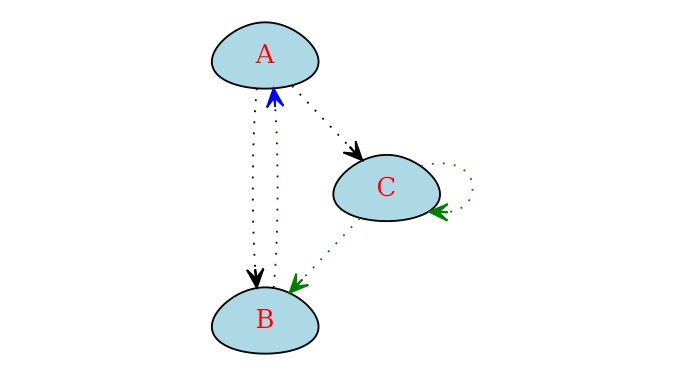
\includegraphics[width=\linewidth]{32.jpeg}
\end{frame}

\begin{frame}[fragile]{DiagrammeR: style = dashed}
\scriptsize
\begin{alltt}
library("DiagrammeR")
grViz("
digraph \{
      node [shape = egg, \hfill # форма узлов
			      fontcolor = red, \hfill # цвет имени узла
			      style = filled, # тип
      fillcolor = lightblue] \hfill # цвет заполнения
      A; B; C \hfill # можно через точку с запятой
      edge [color = black, \hfill # цвет ребра
                 arrowhead = vee, \hfill # конец ребра
{\color{red!13!blue}{                 style = dashed] \hfill # тип линии}}
      A -> {B, C}
      edge [color = blue]   \hfill # цвет ребра
      B -> A 
      edge [color = green] \hfill # цвет ребра
      C -> C C -> B
      \}
      ")
\end{alltt}
\normalsize
\end{frame}
\begin{frame}[fragile]{DiagrammeR: style = dashed}
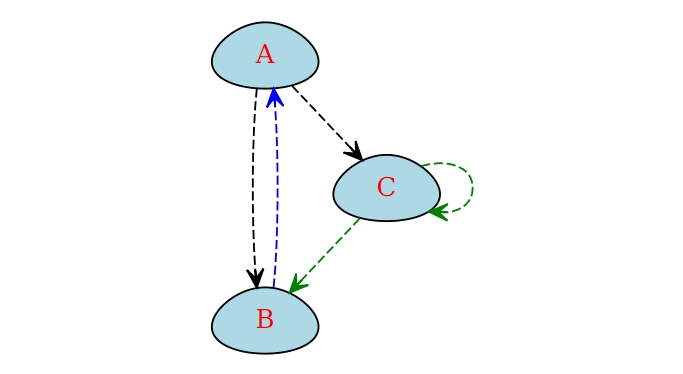
\includegraphics[width=\linewidth]{33.jpeg}
\end{frame}

\begin{frame}[fragile]{DiagrammeR: label}
\scriptsize
\begin{alltt}
library("DiagrammeR")
grViz("
digraph \{
      node [shape = egg, \hfill # форма узлов
			      fontcolor = red, \hfill # цвет имени узла
			      style = filled, # тип
      fillcolor = lightblue] \hfill # цвет заполнения
      A; B; C \hfill # можно через точку с запятой
      edge [color = black, \hfill # цвет ребра
                 arrowhead = vee, \hfill # конец ребра
                 style = dashed] \hfill # тип линии
      A -> {B, C}
      edge [color = blue]   \hfill # цвет ребра
      B -> A 
      edge [color = green] \hfill # цвет ребра
      C -> C C -> B {\color{red!13!blue}{[label = '  tro-lo-lo']}}
      \}
      ")
\end{alltt}
\normalsize
\end{frame}
\begin{frame}[fragile]{DiagrammeR: label}
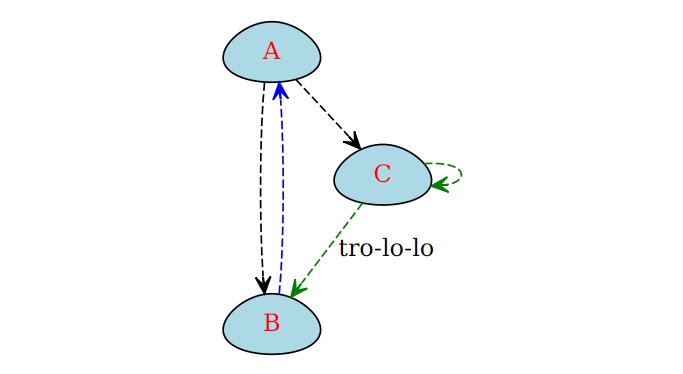
\includegraphics[width=\linewidth]{34.jpeg}
\end{frame}

\begin{frame}[fragile]{DiagrammeR: textcolor = brown}
\scriptsize
\begin{alltt}
library("DiagrammeR")
grViz("
digraph \{
      node [shape = egg, \hfill # форма узлов
			      fontcolor = red, \hfill # цвет имени узла
			      style = filled, # тип
      fillcolor = lightblue] \hfill # цвет заполнения
      A; B; C \hfill # можно через точку с запятой
      edge [color = black, \hfill # цвет ребра
                 arrowhead = vee, \hfill # конец ребра
                 style = dashed] \hfill # тип линии
      A -> {B, C}
      edge [color = blue]   \hfill # цвет ребра
      B -> A 
      edge [color = green] \hfill # цвет ребра
      C -> C C -> B [label = '  tro-lo-lo', {\color{red!13!blue}{textcolor = brown}}]
      \}
      ")
\end{alltt}
\normalsize
\end{frame}
\begin{frame}[fragile]{DiagrammeR: textcolor = brown}
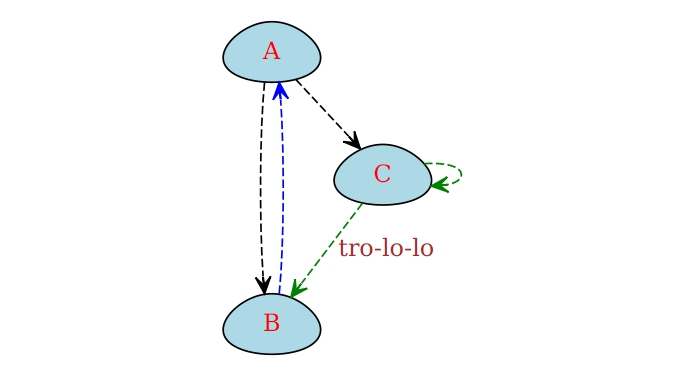
\includegraphics[width=\linewidth]{35.jpeg}
\end{frame}
\section{расположение узлов}
\begin{frame}[fragile]{DiagrammeR: graph [layout = dot]}
\scriptsize
\begin{alltt}
library("DiagrammeR")
grViz("
digraph \{
{\color{red!13!blue}{      graph [layout = dot] \hfill # расположение узлов}}
      node [shape = egg, \hfill # форма узла
      style = filled, \hfill # тип узла
      fillcolor = tomato, \hfill # заполнение узла
      label = ''] \hfill # без имен узлов
      1
      node [fillcolor = green] \hfill # цвет узла
      2; 3; 4
      node [fillcolor = lightblue] \hfill # цвет узла
      5; 6; 7; 8; 9; 10; 11; 12; 13
      1 -> \{2, 3, 4\}
      2 -> \{5, 6\}
      3 -> \{7, 8, 9, 10\}
      4 -> \{11, 12, 13\}
      \}
      ")
\end{alltt}
\normalsize
\end{frame}
\begin{frame}[fragile]{DiagrammeR: graph [layout = dot]}
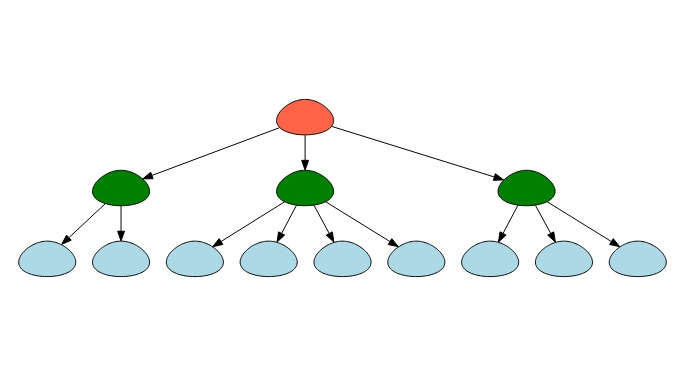
\includegraphics[width=\linewidth]{36.jpeg}
\end{frame}

\begin{frame}[fragile]{DiagrammeR: graph [layout = neato]}
\scriptsize
\begin{alltt}
library("DiagrammeR")
grViz("
digraph \{
{\color{red!13!blue}{      graph [layout = neato] \hfill # расположение узлов}}
      node [shape = egg, \hfill # форма узла
      style = filled, \hfill # тип узла
      fillcolor = tomato, \hfill # заполнение узла
      label = ''] \hfill # без имен узлов
      1
      node [fillcolor = green] \hfill # цвет узла
      2; 3; 4
      node [fillcolor = lightblue] \hfill # цвет узла
      5; 6; 7; 8; 9; 10; 11; 12; 13
      1 -> \{2, 3, 4\}
      2 -> \{5, 6\}
      3 -> \{7, 8, 9, 10\}
      4 -> \{11, 12, 13\}
      \}
      ")
\end{alltt}
\normalsize
\end{frame}
\begin{frame}[fragile]{DiagrammeR: graph [layout = neato]}
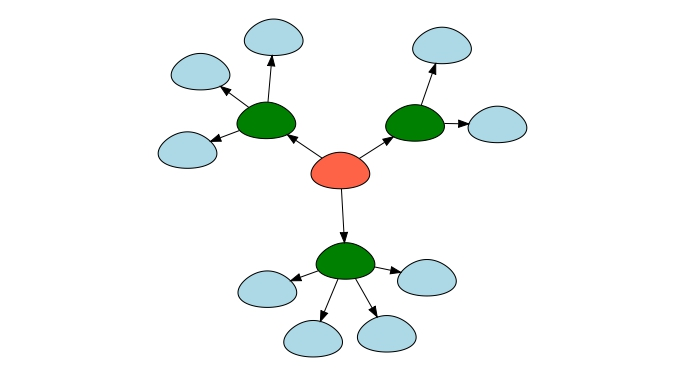
\includegraphics[width=\linewidth]{37.jpeg}
\end{frame}

\begin{frame}[fragile]{DiagrammeR: graph [layout = twopi]}
\scriptsize
\begin{alltt}
library("DiagrammeR")
grViz("
digraph \{
{\color{red!13!blue}{      graph [layout = twopi] \hfill # расположение узлов}}
      node [shape = egg, \hfill # форма узла
      style = filled, \hfill # тип узла
      fillcolor = tomato, \hfill # заполнение узла
      label = ''] \hfill # без имен узлов
      1
      node [fillcolor = green] \hfill # цвет узла
      2; 3; 4
      node [fillcolor = lightblue] \hfill # цвет узла
      5; 6; 7; 8; 9; 10; 11; 12; 13
      1 -> \{2, 3, 4\}
      2 -> \{5, 6\}
      3 -> \{7, 8, 9, 10\}
      4 -> \{11, 12, 13\}
      \}
      ")
\end{alltt}
\normalsize
\end{frame}
\begin{frame}[fragile]{DiagrammeR: graph [layout = twopi]}
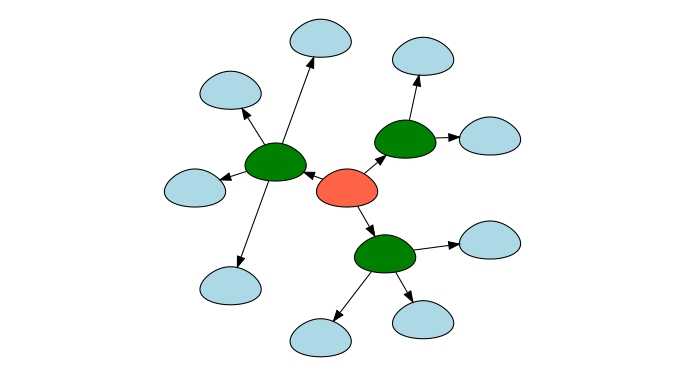
\includegraphics[width=\linewidth]{38.jpeg}
\end{frame}

\begin{frame}[fragile]{DiagrammeR: graph [layout = circo]}
\scriptsize
\begin{alltt}
library("DiagrammeR")
grViz("
digraph \{
{\color{red!13!blue}{      graph [layout = circo] \hfill # расположение узлов}}
      node [shape = egg, \hfill # форма узла
      style = filled, \hfill # тип узла
      fillcolor = tomato, \hfill # заполнение узла
      label = ''] \hfill # без имен узлов
      1
      node [fillcolor = green] \hfill # цвет узла
      2; 3; 4
      node [fillcolor = lightblue] \hfill # цвет узла
      5; 6; 7; 8; 9; 10; 11; 12; 13
      1 -> \{2, 3, 4\}
      2 -> \{5, 6\}
      3 -> \{7, 8, 9, 10\}
      4 -> \{11, 12, 13\}
      \}
      ")
\end{alltt}
\normalsize
\end{frame}
\begin{frame}[fragile]{DiagrammeR: graph [layout = circo]}
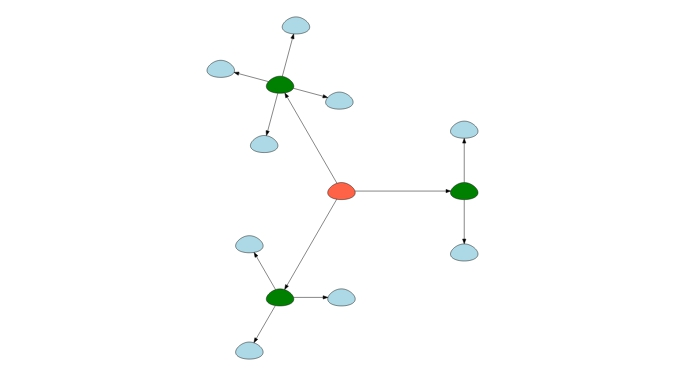
\includegraphics[width=\linewidth]{39.jpeg}
\end{frame}

\section{в Markdown}
\begin{frame}[fragile]{DiagrammeR в Markdown}
\scriptsize
\begin{alltt}
---
title: "DiagrammeR in Markdown"
author: "G. Moroz"
date: "21 января 2016 г."
output: html_document
---

Код DiagrammeR

```\{r, echo=FALSE\}
DiagrammeR::grViz("
                  digraph \{
                          A -> B
                         \}
                  ", height = 200)
```
\end{alltt}
\normalsize
\end{frame}
\begin{frame}[fragile]{DiagrammeR в Markdown}
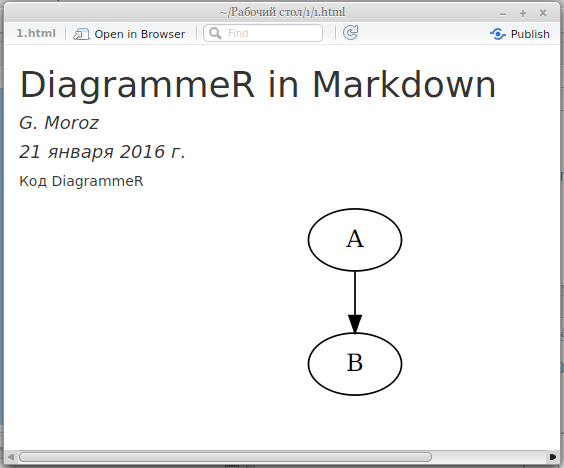
\includegraphics[width=0.8\linewidth]{40.png}
\end{frame}

\section{}
\begin{frame}
{\huge Спасибо за внимание!\bigskip\\
\normalsize Пишите письма\\
agricolamz@gmail.com
\vspace{-130pt}}
\end{frame}
\end{document}